% 抛物线的三种定义

\pentry{圆锥曲线的极坐标方程\upref{Cone}}

\subsection{第二种定义}
我们已经知道用焦点和准线如何定义抛物线, 抛物线的极坐标方程为
\begin{equation}
r = \frac{p}{1 - \cos \theta }
\end{equation}
以与极坐标系相同的原点建立直角坐标系, 要把以上方程变到直角坐标系中, 将$r = \sqrt{x^2 + y^2}$,$\cos \theta  = x/\sqrt{x^2 + y^2}$ 代入得
\begin{equation}
\sqrt{x^2 + y^2}  = p + x
\end{equation}
两边平方并化简得到
\begin{equation}
y^2 = 2p \qty(x + \frac p2)
\end{equation}
把双曲线沿 $x$ 轴正方向移动 $p/2$, 可得标准抛物线方程
\begin{equation}
y^2 = 2px
\end{equation}
所以抛物线的焦距为 $f = p/2$. 与椭圆和双曲线不同的是, 抛物线只有一个自由度即焦距, 所有的抛物线的形状都相似(形状相同, 大小不同).

\subsection{第三种定义}
\begin{figure}[ht]
\centering
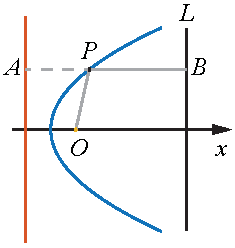
\includegraphics[width=4.2cm]{./figures/Para31.pdf}
\caption{抛物线的第三种定义} \label{Para3_fig1}
\end{figure}

在 $x$ 轴正半轴作一条与准线平行的直线 $L$, 则抛物线上一点 $P$ 到其焦点的距离 $r$ 与 $P$ 到 $L$ 的距离之和不变.

如\autoref{Para3_fig1}, 要证明由焦点和准线定义的抛物线满足该性质, 只需过点 $P$ 作从准线到直线 $L$ 的垂直线段 $AB$, 由于 $r$ 等于线段 $PA$ 的长度, 所以 $r$ 加上 $PB$ 的长度等于 $AB$ 的长度, 与 $P$ 的位置无关. 证毕.
